% Copyright (c) 2022 by Lars Spreng
% This work is licensed under the Creative Commons Attribution 4.0 International License. 
% To view a copy of this license, visit http://creativecommons.org/licenses/by/4.0/ or send a letter to Creative Commons, PO Box 1866, Mountain View, CA 94042, USA.

%~~~~~~~~~~~~~~~~~~~~~~~~~~~~~~~~~~~~~~~~~~~~~~~~~~~~~~~~~~~~~~~~~~~~~~~~~~~~~~
% You can add your packages and commands to the loadslides.tex file. 
% The files in the folder "styles" can be modified to change the layout and design of your slides.
% I have included examples on how to use the template below. 
% Some of it these examples are taken from the Metropolis template.
%~~~~~~~~~~~~~~~~~~~~~~~~~~~~~~~~~~~~~~~~~~~~~~~~~~~~~~~~~~~~~~~~~~~~~~~~~~~~~~


\documentclass[
11pt,notheorems,compress,hyperref={pdfauthor=Maghfira Ramadhani}
]{beamer}


% Copyright (c) 2022 by Lars Spreng
% This work is licensed under the Creative Commons Attribution 4.0 International License. 
% To view a copy of this license, visit http://creativecommons.org/licenses/by/4.0/ or send a letter to Creative Commons, PO Box 1866, Mountain View, CA 94042, USA.

%~~~~~~~~~~~~~~~~~~~~~~~~~~~~~~~~~~~~~~~~~~~~~~~~~~~~~~~~~~~~~~~~~~~~~~~~~~~~~~
% Add your packages and commands to this file
%~~~~~~~~~~~~~~~~~~~~~~~~~~~~~~~~~~~~~~~~~~~~~~~~~~~~~~~~~~~~~~~~~~~~~~~~~~~~~~

%~~~~~~~~~~~~~~~~~~~~~~~~~~~~~~~~~~~~~~~~~~~~~~~~~~~~~~~~~~~~~~~~~~~~~~~~~~~~~~
\RequirePackage{palatino}
\RequirePackage[utf8]{inputenc}
\RequirePackage[T1]{fontenc}

\usefonttheme{serif}

\usepackage{styles/elegantmacros}
\usefolder{styles}
\usetheme[style=blue]{elegant}

\newcommand{\makepart}[1]{ % For convenience
\part{#1} \frame{\partpage}
}

%~~~~~~~~~~~~~~~~~~~~~~~~~~~~~~~~~~~~~~~~~~~~~~~~~~~~~~~~~~~~~~~~~~~~~~~~~~~~~~

%~~~~~~~~~~~~~~~~~~~~~~~~~~~~~~~~~~~~~~~~~~~~~~~~~~~~~~~~~~~~~~~~~~~~~~~~~~~~~~
% Figures
\RequirePackage{booktabs}
\RequirePackage{colortbl}
\RequirePackage{ragged2e}
\RequirePackage{schemabloc}
%\RequirePackage{natbib}
\RequirePackage{caption}
\RequirePackage{subcaption}
\RequirePackage{tabularx}
\RequirePackage{array}
\RequirePackage{multirow}
\usepackage[
  style=authoryear, 
]{biblatex}
\addbibresource{references.bib}
\newcolumntype{Y}{>{\centering\arraybackslash}X}

%~~~~~~~~~~~~~~~~~~~~~~~~~~~~~~~~~~~~~~~~~~~~~~~~~~~~~~~~~~~~~~~~~~~~~~~~~~~~~~

%~~~~~~~~~~~~~~~~~~~~~~~~~~~~~~~~~~~~~~~~~~~~~~~~~~~~~~~~~~~~~~~~~~~~~~~~~~~~~~
% Figures
\RequirePackage{wrapfig}
\RequirePackage{pgfplots}
\RequirePackage{graphicx}
\RequirePackage{adjustbox}
\RequirePackage{environ}
\pgfplotsset{compat=1.18}

\makeatletter
\newsavebox{\measure@tikzpicture}
\NewEnviron{scaletikzpicturetowidth}[1]{%
  \def\tikz@width{#1}%
  \def\tikzscale{1}\begin{lrbox}{\measure@tikzpicture}%
  \BODY
  \end{lrbox}%
  \pgfmathparse{#1/\wd\measure@tikzpicture}%
  \edef\tikzscale{\pgfmathresult}%
  \BODY
}
\makeatother
%~~~~~~~~~~~~~~~~~~~~~~~~~~~~~~~~~~~~~~~~~~~~~~~~~~~~~~~~~~~~~~~~~~~~~~~~~~~~~~

%~~~~~~~~~~~~~~~~~~~~~~~~~~~~~~~~~~~~~~~~~~~~~~~~~~~~~~~~~~~~~~~~~~~~~~~~~~~~~~
% Maths 
\RequirePackage{textcomp}
\RequirePackage{amsmath} 
\RequirePackage{amsthm}
\RequirePackage{mathtools}
%\RequirePackage{bbm}
%\RequirePackage{algorithm}
%\RequirePackage[osf,sc]{mathpazo}
%\RequirePackage{pifont}
%\newcommand{\xmark}{\ding{55}}%
%\numberwithin{equation}{section}
\DeclareMathOperator*{\argmax}{arg\,max}
\DeclareMathOperator*{\argmin}{arg\,min}

\setbeamertemplate{theorems}[numbered] % to number

\theoremstyle{definition}
\newtheorem{fact}{Fact}[section]
\newtheorem{examp}{Example}[section]

\theoremstyle{plain}
\newtheorem{definition}{Definition}[section]
\newtheorem{proposition}{Proposition}
\newtheorem{theorem}{Theorem}
\newtheorem{assumption}{Assumption}

\providecommand{\H}{\mathscr{H}}      
\providecommand{\E}{\mathbb{E}}
\makeatletter
\def\munderbar#1{\underline{\sbox\tw@{$#1$}\dp\tw@\z@\box\tw@}}
\makeatother

%~~~~~~~~~~~~~~~~~~~~~~~~~~~~~~~~~~~~~~~~~~~~~~~~~~~~~~~~~~~~~~~~~~~~~~~~~~~~~~
 % Loads packages and some defined commands

\title[
% Text entered here will appear in the bottom middle
]{Improving Rural Accessibility in Indonesia: Fuel Subsidy versus Infrastructure Development}

\author[
% Text entered here will appear in the bottom left corner
]{
    Maghfira Ramadhani 
}

\institute{
    School of Economics, \\
    Georgia Institute of Technology}
\date{\today}

\begin{document}

% Generate title page
{
\setbeamertemplate{footline}{}
\begin{frame}
  \titlepage
\end{frame}
}
\addtocounter{framenumber}{-1}

% You can declare different parts as a parentof sections

{
\setbeamertemplate{footline}{}
\begin{frame}{Outline}
    \tableofcontents%[part=1]
\end{frame}
}
%\makepart{Proposal}
\section{Introduction}
\begin{frame}
\setbeamercovered{transparent}
\begin{columns}[T,onlytextwidth]
    \column{0.7\textwidth}
\onslide<1->{\begin{block}{Motivation}
\begin{itemize}
    \item Indonesia has been subsidizing fuel for a long time, but high fuel prices in rural areas were observed in the last decade. 
    \item Linking underdeveloped regions to growth centers is a challenge.
    \item One Price Fuel program started in 2016 to guarantee the availability of subsidized fuel at the same price control.
    \item Political economy perspective of infrastructure development vs. fossil fuel subsidy \citep{ichsan_2022,ichsan_2021}.
\end{itemize}
\end{block}}
\onslide<2->{\begin{block}{Research Question}
\begin{itemize}
    \item Does the fuel policy improve accessibility in rural areas?
    \item Which policy option is more efficient?
\end{itemize}
\end{block}}
    \column{0.3\textwidth}
    \onslide<1->{\begin{figure}[t]
        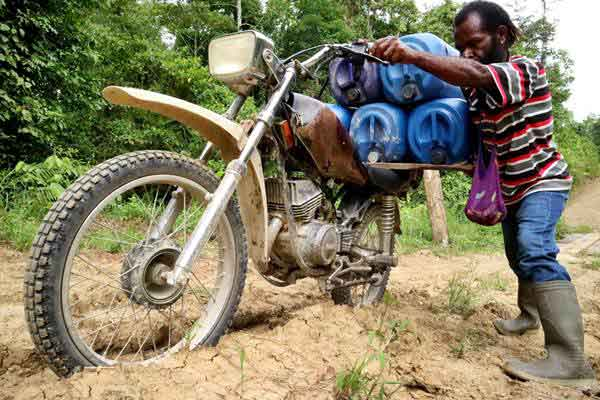
\includegraphics[scale=0.21]
        {Final_Project/image/bbm-papua-221017.jpg}
        \end{figure}
    \begin{figure}[t]
        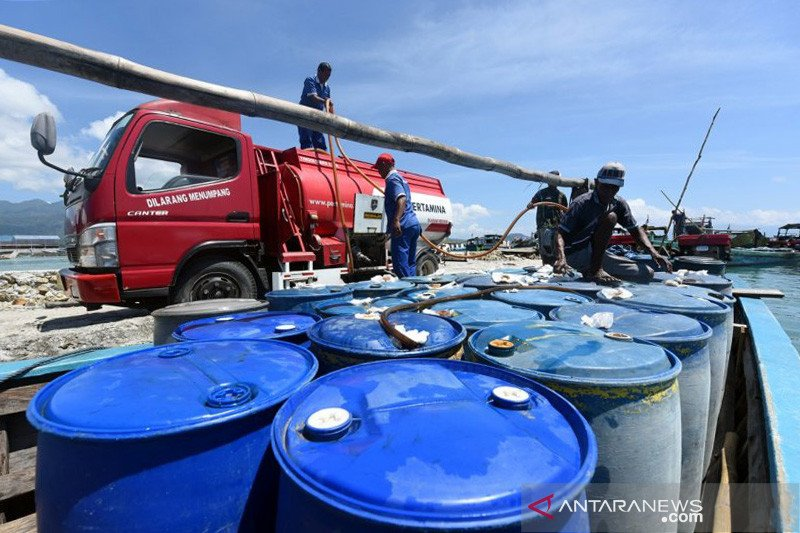
\includegraphics[scale=0.21]
        {Final_Project/image/bbm-satu-harga_1.jpg}
        \end{figure}}
\end{columns}
\end{frame}

\section{Institutional Context and Conceptual Framework}
\subsection{Accessibility in rural area}
\begin{frame}
\setbeamercovered{transparent}
\onslide<1->{\begin{block}{Transportation cost in rural area}
\begin{itemize}
    \item Transportation spending \al{dominates energy spending} \citep{sambodo_2019}
    \item The \al{lack of adequate and reliable infrastructure} drives up the transportation cost \citep{sandee_2016}.
    \item We can treat unit transportation cost as the \alg{willingness to pay} or demand for transportation
\end{itemize}
\end{block}}
\onslide<2->{\begin{block}{Demand theory of transportation}
\begin{itemize}
    \item We follow previous literature on WTP for rural transportation from revealed preference, the affecting factors include \al{travel time, convenience}, and \al{trip purpose} i.e. work or education.   
\end{itemize}
\end{block}}
\end{frame}

\subsection{Fossil fuel subsidy regime}
\begin{frame}
    \begin{columns}[T,onlytextwidth]
    \column{0.5\textwidth}
      \begin{figure}[t]
        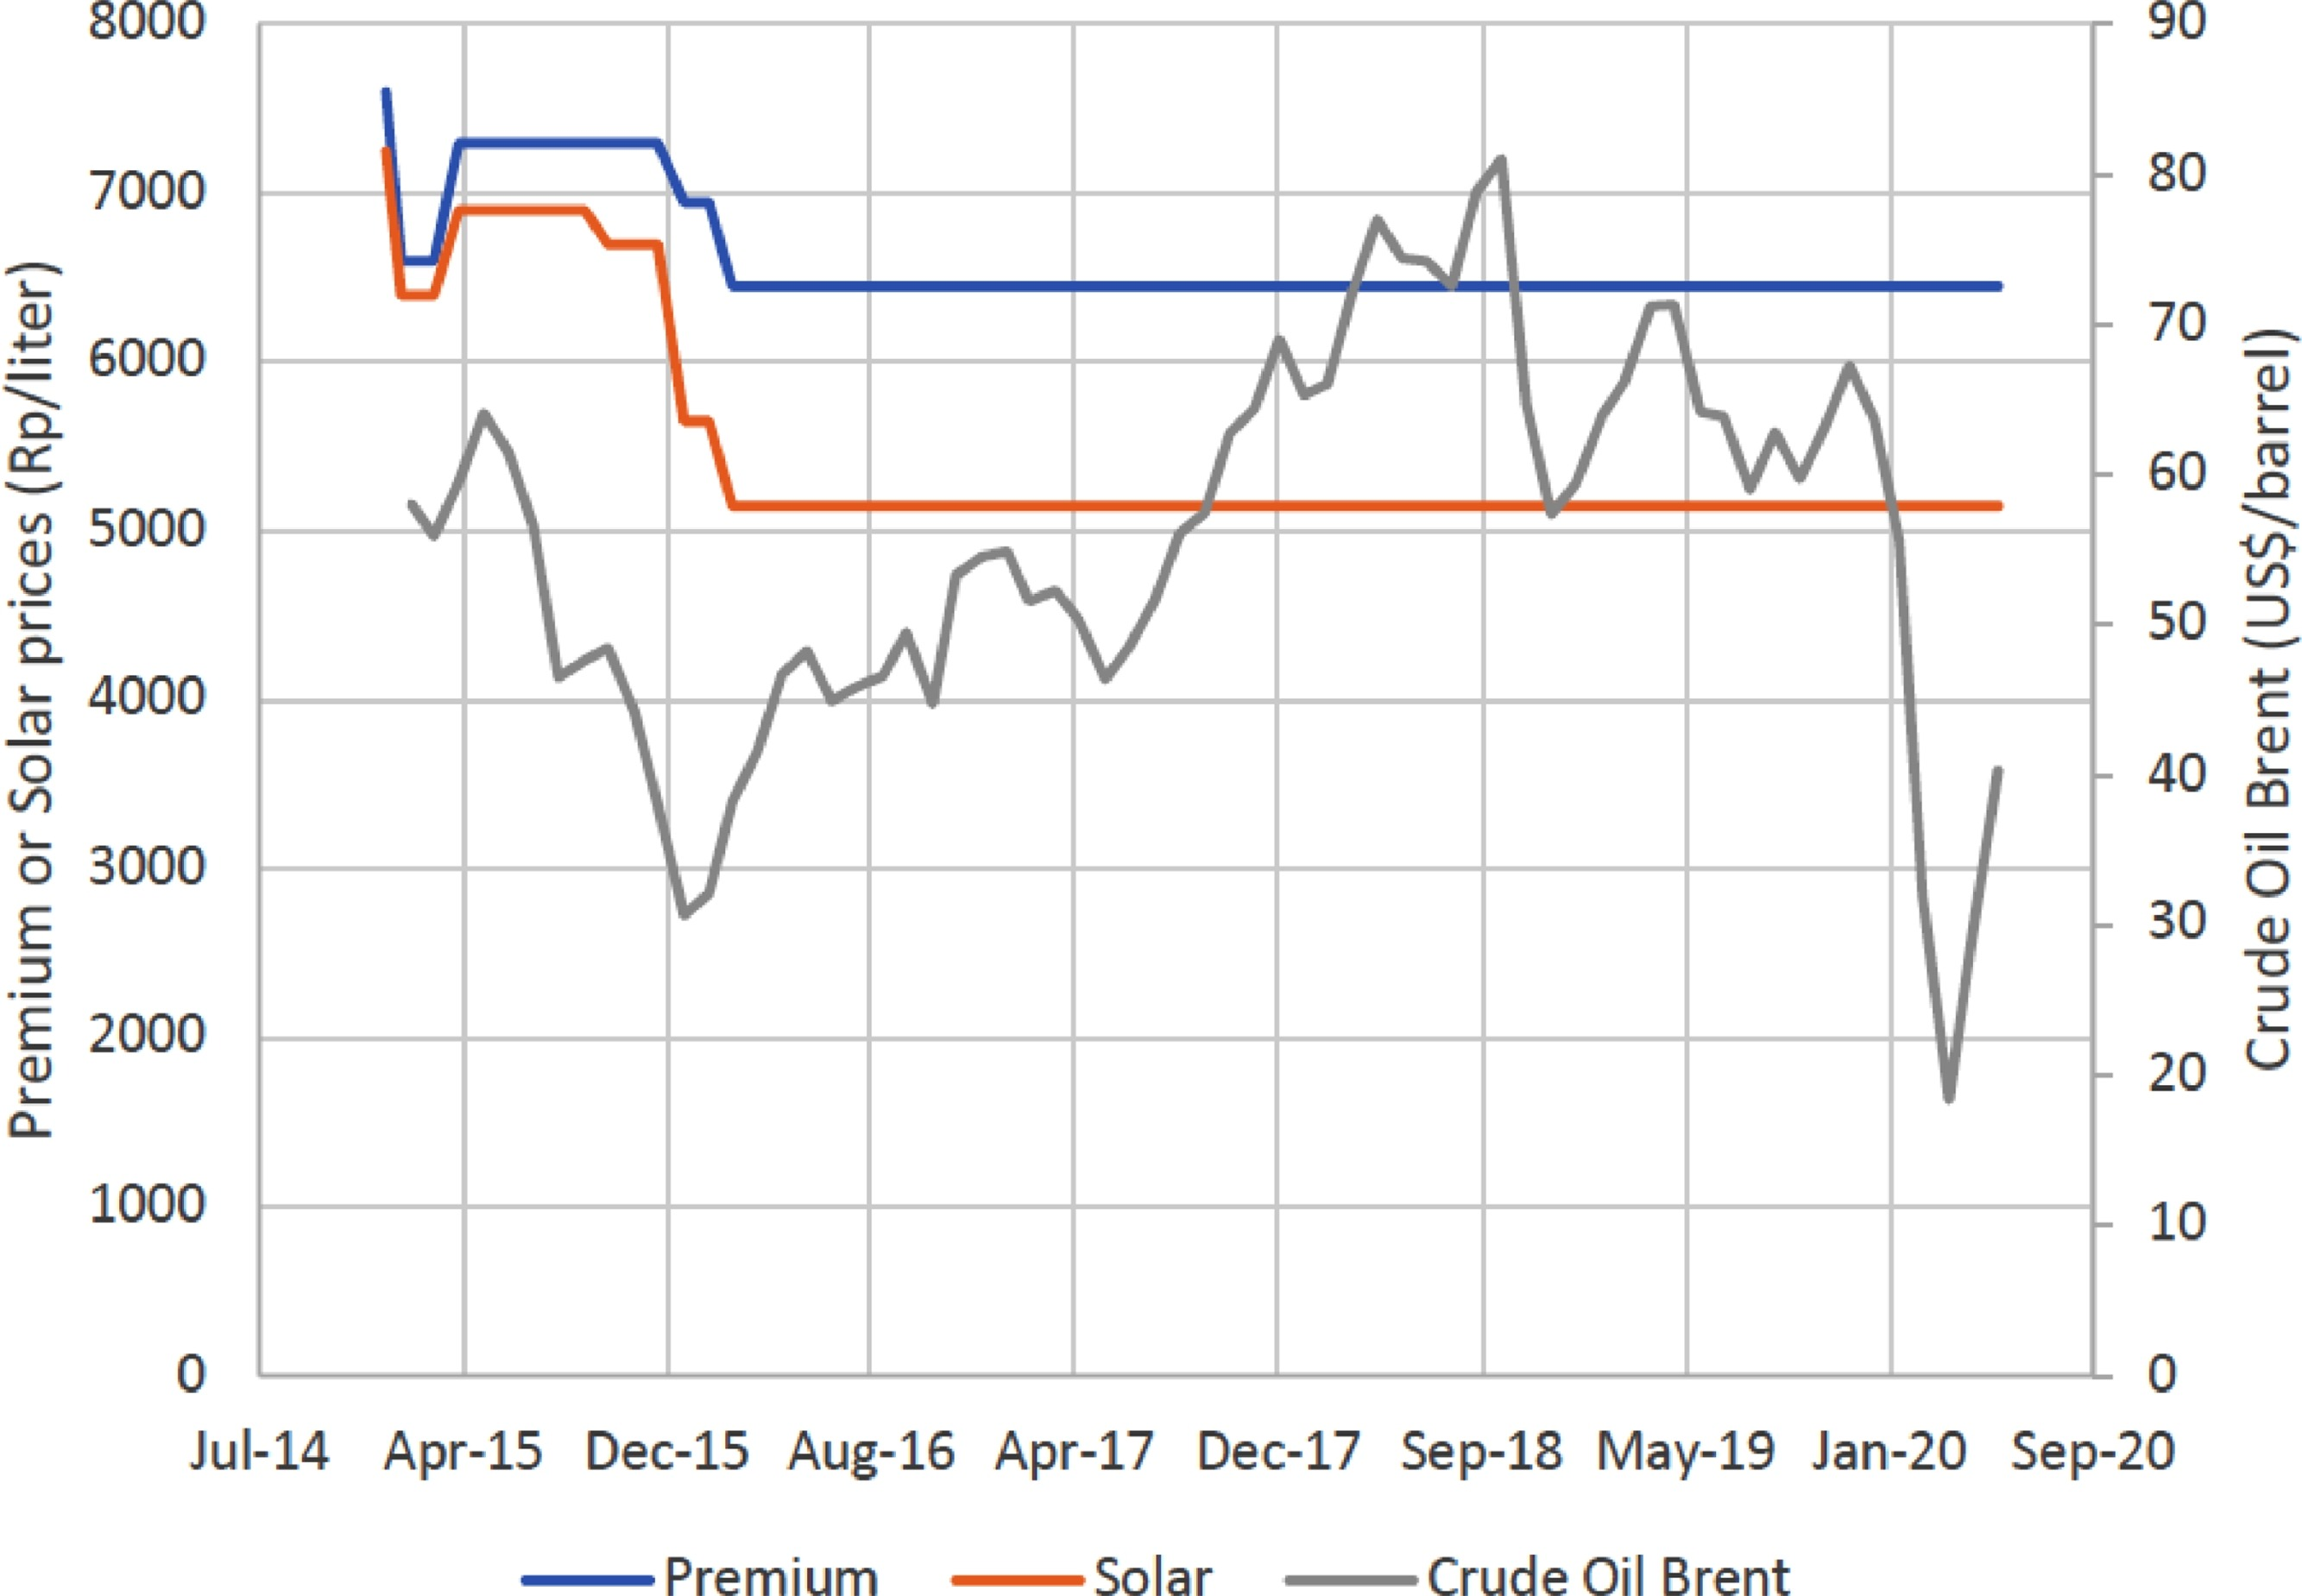
\includegraphics[scale=0.52]{Final_Project/image/bbm-price-2014-2018.jpg}
        \caption{Fuel Price Control 2014-2018}
        \label{f:graph1}
        \end{figure}
        \begin{itemize}
            \item The price control regime implies variation in transportation costs in rural areas is due to \al{distributional problems}.
        \end{itemize}
    \column{0.5\textwidth}
        \begin{figure}[t]
        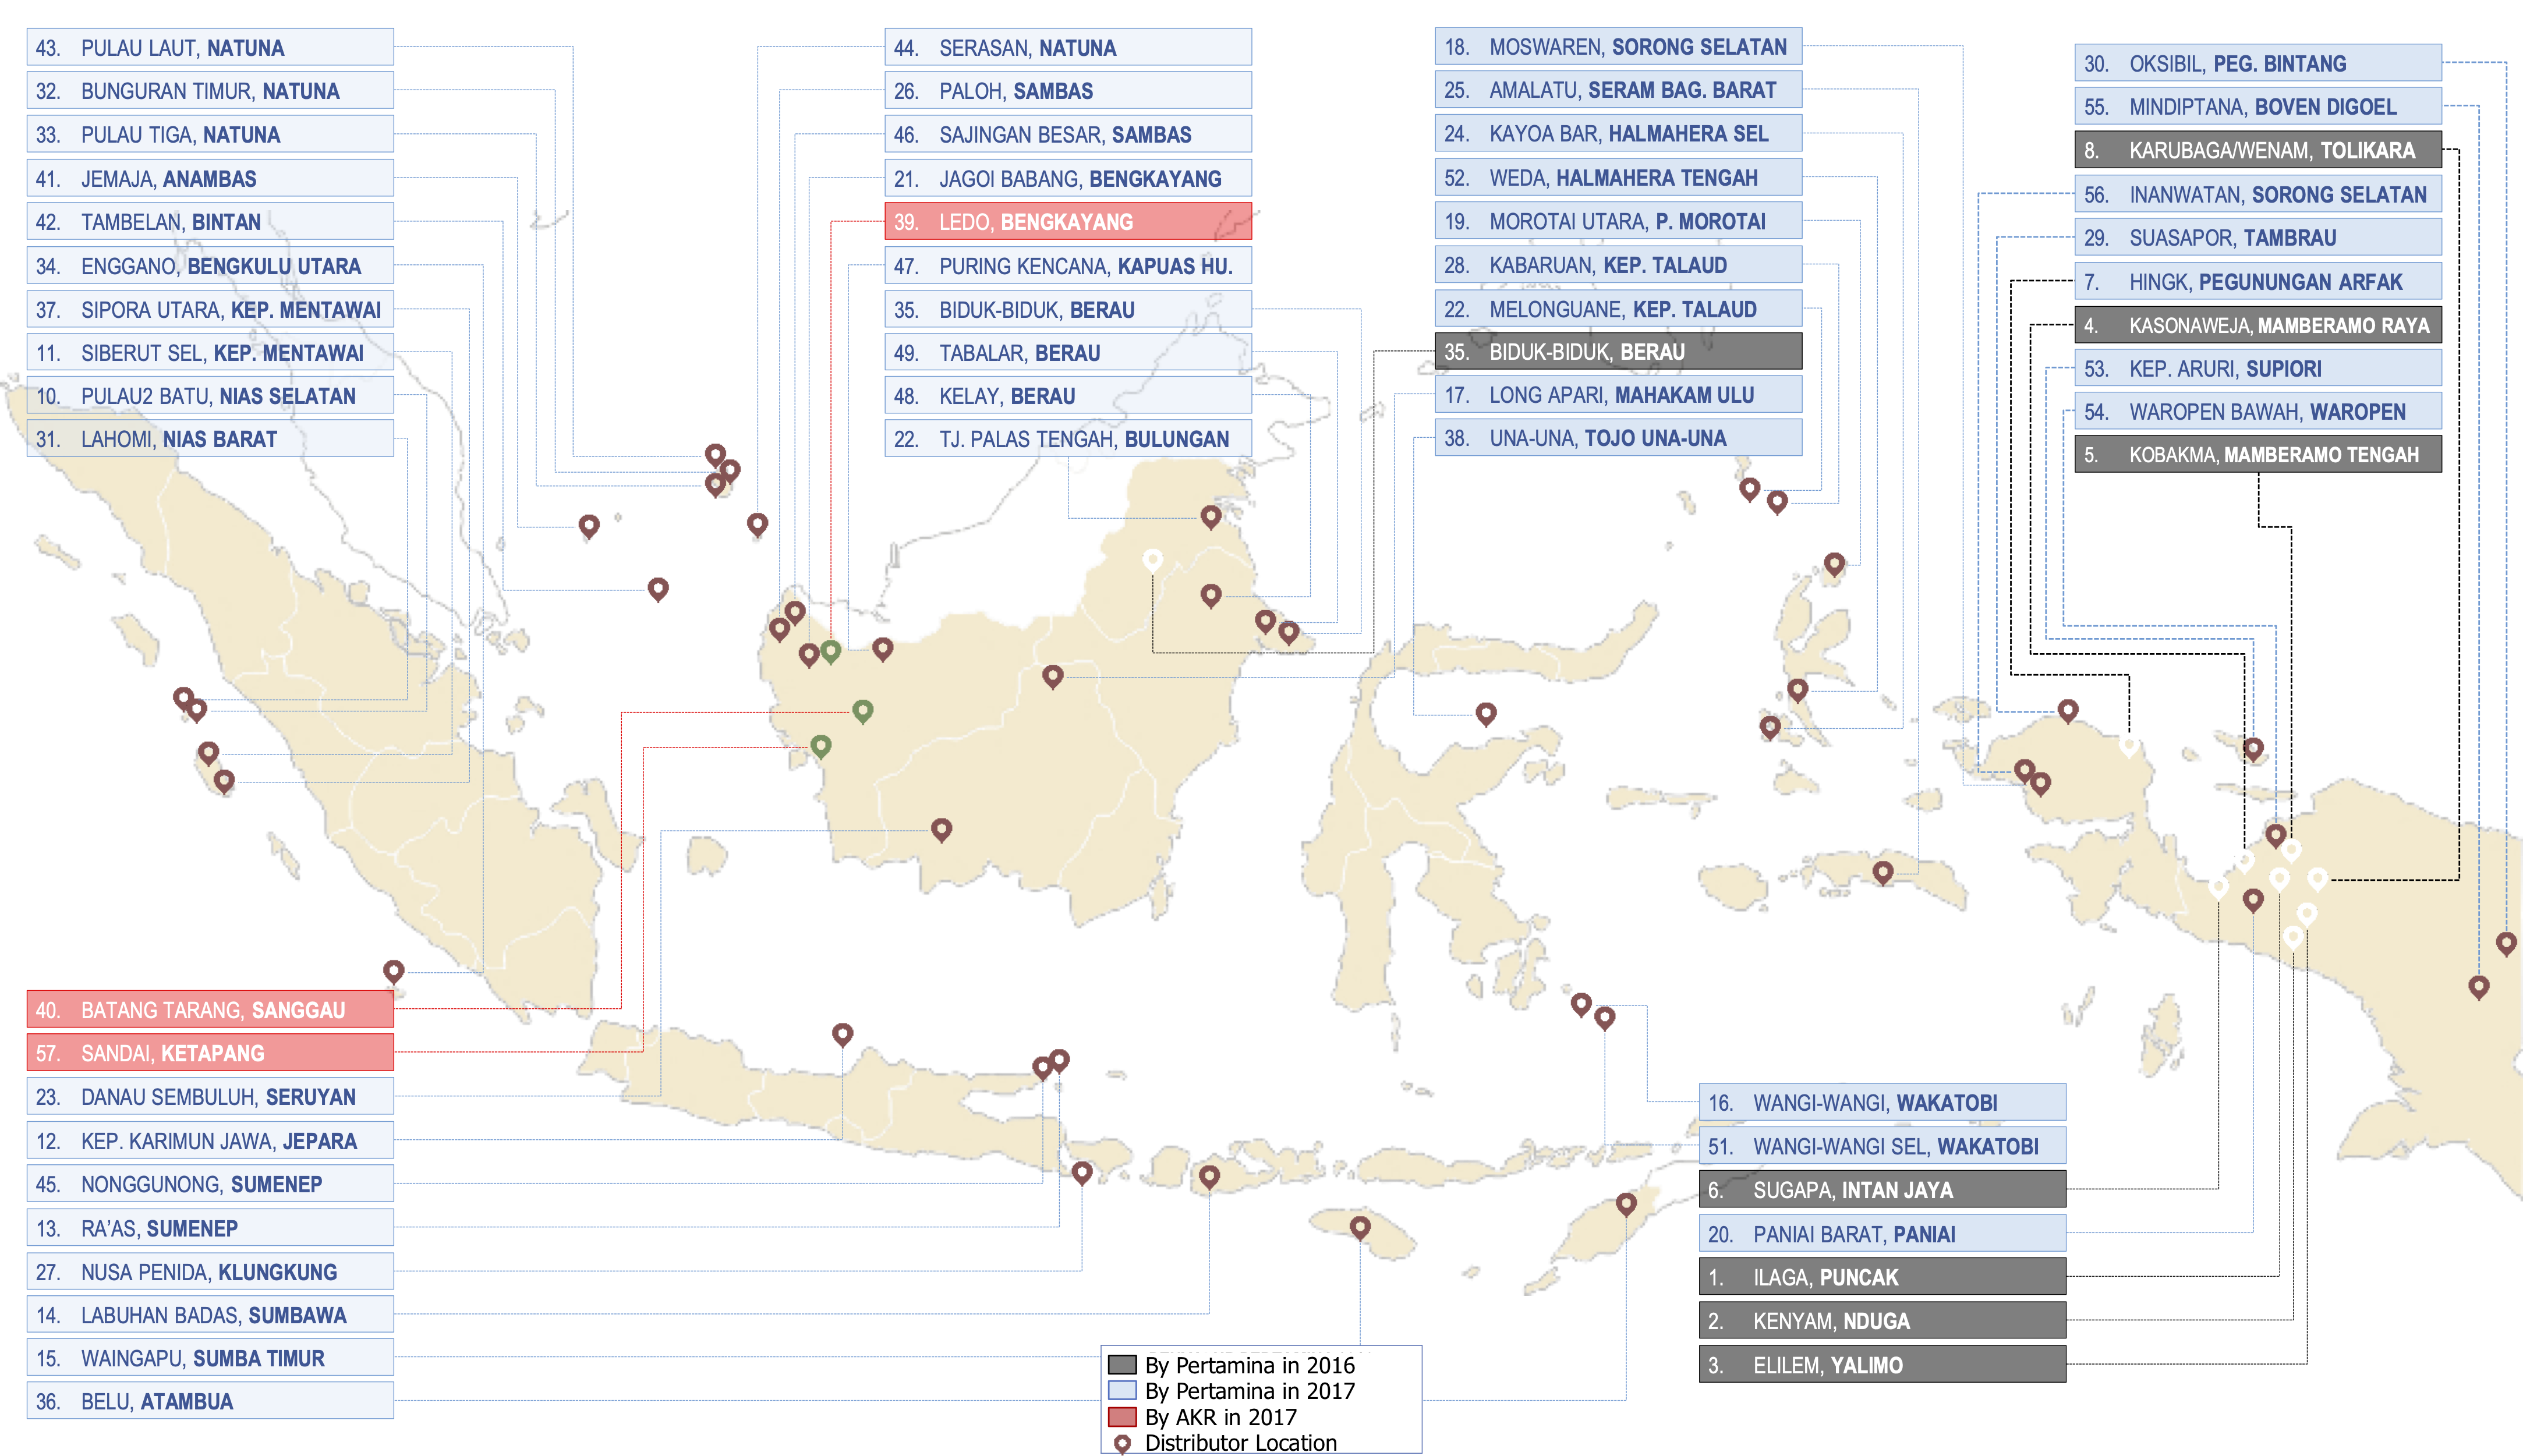
\includegraphics[scale=0.305]{Final_Project/image/BBM Satu Harga.png}
        \caption{Location of the Program in 2016-2017}
        \label{f:graph2}
        \end{figure}
        \begin{itemize}
            \item The location choice of intervention \al{is not randomly assigned}, as they targeted the outermost underdeveloped region.
        \end{itemize}
    \end{columns}
\end{frame}

\subsection{Decentralization of development}
\begin{frame}\setbeamercovered{transparent}
    \begin{columns}[T,onlytextwidth]
    \column{0.5\textwidth}
      \begin{figure}[t]
        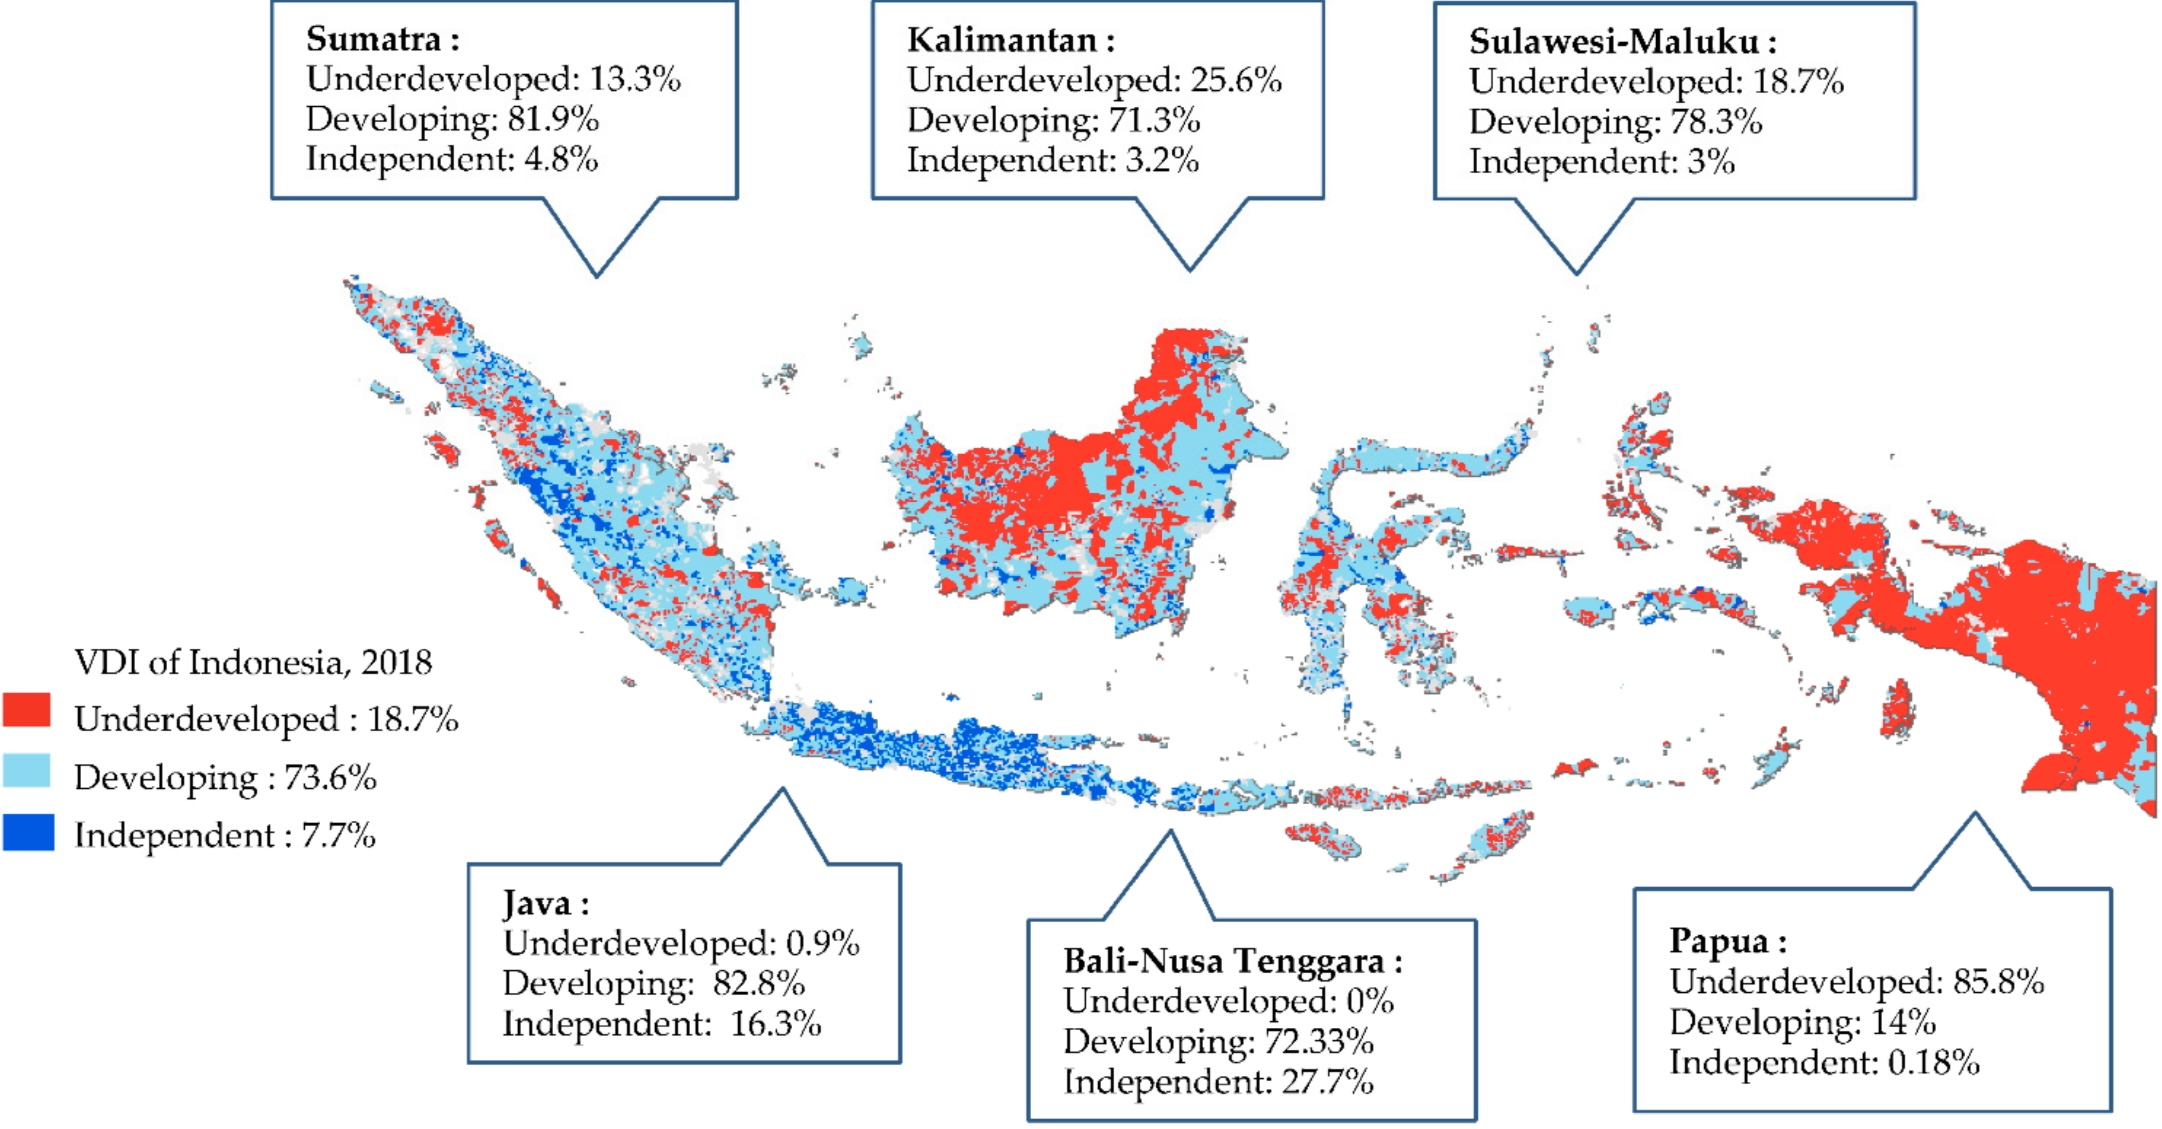
\includegraphics[scale=0.205]{Final_Project/image/vdi2018.jpg}
        \caption{Indonesia's VDI's status}
        \label{f:graph3}
        \end{figure}
    \column{0.5\textwidth}
        \begin{itemize}
            \item Developing countries believe \alg{decentralization and local government reform} are \alert{\textbf{more efficient}} in bringing local development \citep{vazquez_2017} and \al{providing public goods better} that central government \citep{arends2020}.
            \pause\item In 2014 the government enacted \al{village fund transfer} to implement decentralization at the village level\footnote{See Village Law No. 6 of 2014}. The allocation amount takes into account village conditions, i.e. poverty and geographic difficulty into account.
        \end{itemize}
    \end{columns}
\end{frame}

\section{Data}
\subsection{Data Description}
\begin{frame}
\setbeamercovered{transparent}
    \begin{itemize}
        \item I obtained the \al{Village Potential Statistics} data for the years 2014 and 2018 from Indonesia's Central Bureau of Statistics complemented with village fund transfer data from the Ministry of Village Development.
        \pause\item I measure rural accessibility using the \al{unit transportation cost} (in Rp/km) of each individual village $i$ for year $t$. 
        \footnote{I define \al{unit transportation cost}, $y_{it}$, as the \al{transportation cost} from the village $i$'s office to the sub-district office (in thousands Rp) at year $t$, $c_{it}$, divided by the \al{distance} from the village office $i$'s to the sub-district office (in km) at year $t$, $d_{it}$.
        \begin{equation}
        y_{it}=\frac{d_{it}}{c_{it}}    
        \end{equation}}
        \pause\item I obtain the list of 55 government-appointed new distributor's village locations from the NOC and then define all the villages that are in the same sub-district as the \al{treated} by the program, i.e. $D_{it}=1$ in the year 2018. Note in the year 2014 all $D_{it}=0$. 
        \begin{itemize}
            \item \alg{For example}, suppose the government in 2016 gives the order for the NOC to build a new distribution point at village $A$. Village $A$ is in the same sub-district as villages $B,C$, and $D$. Then all villages $A,B,C$, and $D$ are treated.
        \end{itemize}
        \pause\item Other data on geographic characteristics, i.e land topography, region boundary with forest or sea, river transportation use, and poverty can be used as covariates or instruments.
    \end{itemize}
\end{frame}

\subsection{Summary Statistics}
\begin{frame}
    \begin{table}[h]
    \caption{Summary statistics of main variables. }
    \scalebox{0.75}{\begin{tabular}{l*{2}{ccccc}}
\toprule
                &     2014&         &         &         &         &     2018&         &         &         &         \\
                &     Mean&     S.D.&      Min&      Max&     Obs.&     Mean&     S.D.&      Min&      Max&     Obs.\\
\midrule
\emph{Transportation Cost}&         &         &         &         &         &         &         &         &         &         \\
\hspace{0.25cm} Unit transportation cost in 000s Rp./km&     5.14&    21.02&     0.00&  1000.00&     3407&     4.93&    12.47&     0.00&   400.00&     3411\\
\hspace{0.25cm} Travel Duration&     1.27&     1.27&     1.00&    30.00&     3407&     0.74&     2.36&     0.00&    60.50&     3411\\
\vspace{0.05em} \\ \emph{Natural Disaster}&         &         &         &         &         &         &         &         &         &         \\
\hspace{0.25cm} Landfall occurence average per year&     0.07&     0.37&     0.00&     6.00&     3407&     0.10&     0.49&     0.00&     9.00&     3411\\
\hspace{0.25cm} Earthquake occurence average per year&     0.04&     0.35&     0.00&     7.00&     3407&     0.46&     1.60&     0.00&     9.00&     3411\\
\vspace{0.05em} \\ \emph{Infrastructure}&         &         &         &         &         &         &         &         &         &         \\
\hspace{0.25cm} Number of PLN electricity user household&   366.92&   610.20&     0.00&  6726.00&     3407&   422.79&   651.77&     0.00&  6468.00&     3411\\
\hspace{0.25cm} Number of Junior High School&     0.54&     0.85&     0.00&     9.00&     3407&     0.61&     0.89&     0.00&    12.00&     3411\\
\hspace{0.25cm} Number of Senior High School&     0.27&     0.66&     0.00&     7.00&     3407&     0.33&     0.73&     0.00&     8.00&     3411\\
\vspace{0.05em} \\ \emph{Inter-government Transfer}&         &         &         &         &         &         &         &         &         &         \\
\hspace{0.25cm} Revenue from village fund transfer&   113.55&   129.92&     0.00&  1253.00&     3407&   158.93&   289.35&     0.00& 13662.00&     3172\\
\bottomrule
\end{tabular}
}
    \label{t1}\end{table}
\end{frame}

\section{Empirical Strategy}
\subsection{Identification and Model Specification}
\begin{frame}
\begin{itemize}
    \item Serial correlation should not be an issue since the panel is 4 years apart.
    \item Following \citet{hausman78}, the specification test suggest using \al{fixed effects}. \hyperlink{hausmanspec}{\beamergotobutton{Hausman test}}\label{hausmanclick}
    \item Possible \al{endogeneity treat} from Village Fund Transfer $(VF_{it})$ and Treatment $(D_{it})$, therefore I need to identify whether there is a good instrument available in the datasets. \hyperlink{FSVF}{\beamergotobutton{$VF_{it}$}}\label{VFclick}\hyperlink{FSD}{\beamergotobutton{$D_{it}$}}\label{Dclick}
    \item Following \citet{abadie2016}, I can use \al{Propensity Score Matching} to construct an artificial control group by matching each treated unit with a non-treated unit of similar characteristics.
    \item I follow the following model specification
    \begin{equation}
    \resizebox{.6\textwidth}{!}{%
        y_{it}=\alpha_i+\theta_t+\delta_1 D_{it}+\gamma_1 VF_{it}+\textbf{X}\pmb{\beta}+\varepsilon_{it}\label{ppt2}
    }%
    \end{equation}
    where $y_{it}$ represents the unit transportation cost in village $i$ in year $t$,
    $\alpha_i$ represents the village fixed effects, $\theta_t$ represents time trend or time fixed effects, $D_{it}$ and $VF_{it}$ is the main variable of interests, and $\textbf{X}$ as vector of covariates.
    \item \al{Fixed Effect Instrumental Variable} (FEIV) approach (similar to FDIV for $T=2$) can be applied to identify $\delta_1$ and $\gamma_1$ in equation \eqref{ppt2}.
    \end{itemize}
\end{frame}


\section{Results}
\subsection{Main Findings}
\begin{frame}
\setbeamercovered{transparent}
    \begin{block}{Findings 1}
        Block content.
    \end{block}
    \pause\begin{block}{Findings 2}
        Block content.
    \end{block}
    \pause\begin{block}{Findings 3}
        Block content.
    \end{block}
\end{frame}

\subsection{Robustness}
\begin{frame}
    \begin{columns}[T,onlytextwidth]
    \column{0.33\textwidth}
      \textbf{Items}
      \begin{itemize}
        \item Cats 
        \begin{itemize}
            \item British Shorthair
        \end{itemize}
        \item Dogs \item Birds
      \end{itemize}

    \column{0.33\textwidth}
      \textbf{Enumerations}
      \begin{enumerate}
        \item First 
        \begin{enumerate}
            \item First subpoint
        \end{enumerate}
        \item Second \item Last
      \end{enumerate}

    \column{0.33\textwidth}
      \textbf{Descriptions}
      \begin{description}
        \item[Apples] Yes \item[Oranges] No \item[Grappes] No
      \end{description}
\end{columns}
\end{frame}

\subsection{Cost-Benefit Analysis}
\begin{frame}
    
\end{frame}

\section{Concluding Remarks}
\begin{frame}
    \begin{table}
        \caption{Largest cities in the world (source: Wikipedia)}
        \begin{tabular}{@{} lr @{}}
          \toprule
          City & Population\\
          \midrule
          Mexico City & 20,116,842\\
          Shanghai & 19,210,000\\
          Peking & 15,796,450\\
          Istanbul & 14,160,467\\
          \bottomrule
        \end{tabular}
        \hspace*{1cm}
            \setlength\extrarowheight{3pt}
        \begin{tabular}{|lr|}
          \hline
          \rowcolor{primary}\color{white}City & \color{white}Population\\
          \hline
          Mexico City & 20,116,842\\
          Shanghai & 19,210,000\\
          Peking & 15,796,450\\
          Istanbul & 14,160,467\\
          \hline
        \end{tabular}
    \end{table}
\end{frame}

\section{}
\begin{frame}[allowframebreaks]{References}
    \bibliographystyle{Final_Project/paper/bibliography.bst}
    \bibliography{references.bib}
\end{frame}

\begin{frame}{}
  \centering
  {\LARGE\emph{Thank you!}}\\
  \vspace{1cm}
  Any Comments, Suggestions, Ideas\\
  \href{mailto:\maghfira.ramadhani@gatech.edu}{\faEnvelope\ \  \al{maghfira.ramadhani@gatech.edu}}\\
  \href{http://maghfiraer.github.io}{\faHome\ \  \al{maghfiraer.github.io}} \\
  \href{https://github.com/maghfiraer/ECON7023-Metrics-II/tree/main/Final_Project}{\faGithubSquare\ \  \al{Replication Code}}
\end{frame}

\appendix
\section{Appendix}
\subsection{First Stage Regression}
\begin{frame}
\label{FSVF}
    \begin{table}[h]
    \caption{First Stage Regression on Village Fund Transfer \hyperlink{VFclick}{\beamerreturnbutton{Back}}}
    \scalebox{0.6}{{
\def\sym#1{\ifmmode^{#1}\else\(^{#1}\)\fi}
\begin{tabular}{l*{5}{c}}
\toprule
                    &\multicolumn{1}{c}{(1)}         &\multicolumn{1}{c}{(2)}         &\multicolumn{1}{c}{(3)}         &\multicolumn{1}{c}{(4)}         &\multicolumn{1}{c}{(5)}         \\
\midrule
Number of poverty statement request&       0.001\sym{***}&       0.001\sym{**} &       0.001\sym{**} &       0.001\sym{**} &       0.001\sym{**} \\
                    &     (0.000)         &     (0.000)         &     (0.000)         &     (0.000)         &     (0.000)         \\
\addlinespace
Number of PLN electricity user household&                     &       0.009\sym{***}&       0.009\sym{***}&       0.015\sym{***}&       0.014\sym{***}\\
                    &                     &     (0.001)         &     (0.001)         &     (0.001)         &     (0.001)         \\
\addlinespace
Earthquake frequency [y-1]&                     &                     &       0.357         &       1.348\sym{***}&       0.923\sym{**} \\
                    &                     &                     &     (0.452)         &     (0.435)         &     (0.435)         \\
\addlinespace
=1 if slope/valleys, =0 vast land&                     &                     &                     &      -7.731\sym{***}&                     \\
                    &                     &                     &                     &     (1.381)         &                     \\
\addlinespace
=1 if inside or border with forest, =0 outside forest&                     &                     &                     &      13.153\sym{***}&                     \\
                    &                     &                     &                     &     (1.441)         &                     \\
\addlinespace
=1 if border with sea, =0 no border with sea&                     &                     &                     &      27.160\sym{***}&      28.802\sym{***}\\
                    &                     &                     &                     &     (1.824)         &     (1.780)         \\
\addlinespace
=1 if river used for transportation, =0 otherwise&                     &                     &                     &      65.724\sym{***}&      70.268\sym{***}\\
                    &                     &                     &                     &     (3.883)         &     (3.760)         \\
\addlinespace
Constant            &     120.111\sym{***}&     114.038\sym{***}&     113.977\sym{***}&      97.267\sym{***}&      99.125\sym{***}\\
                    &     (0.625)         &     (0.863)         &     (0.881)         &     (1.204)         &     (0.949)         \\
\midrule
Observations        &       87842         &       87842         &       87842         &       87842         &       87842         \\
\(R^{2}\)           &       0.000         &       0.002         &       0.002         &       0.017         &       0.016         \\
Adjusted \(R^{2}\)  &       0.000         &       0.002         &       0.002         &       0.017         &       0.016         \\
F                   &       8.047         &      55.568         &      37.051         &     134.336         &     136.159         \\
\bottomrule
\multicolumn{6}{l}{\footnotesize Standard errors in parentheses}\\
\multicolumn{6}{l}{\footnotesize \sym{*} \(p<0.10\), \sym{**} \(p<0.05\), \sym{***} \(p<0.01\)}\\
\end{tabular}
}
}    
    \end{table}
\end{frame}

\begin{frame}
\label{FSD}
    \begin{table}[h]
    \caption{First Stage Regression on Treatment \hyperlink{Dclick}{\beamerreturnbutton{Back}}}
    \scalebox{0.55}{{
\def\sym#1{\ifmmode^{#1}\else\(^{#1}\)\fi}
\begin{tabular}{l*{5}{c}}
\toprule
                    &\multicolumn{1}{c}{(1)}         &\multicolumn{1}{c}{(2)}         &\multicolumn{1}{c}{(3)}         &\multicolumn{1}{c}{(4)}         &\multicolumn{1}{c}{(5)}         \\
\midrule
\hspace{0.25cm} Number of poverty statement request&      -0.000\sym{***}&       0.000         &      -0.000         &      -0.000         &      -0.000         \\
                    &     (0.000)         &     (0.000)         &     (0.000)         &     (0.000)         &     (0.000)         \\
\addlinespace
\hspace{0.25cm} Number of PLN electricity user household&                     &      -0.000\sym{***}&      -0.000\sym{***}&      -0.000\sym{***}&      -0.000\sym{***}\\
                    &                     &     (0.000)         &     (0.000)         &     (0.000)         &     (0.000)         \\
\addlinespace
\hspace{0.25cm} Earthquake occurence average per year&                     &                     &       0.002\sym{***}&       0.002\sym{***}&       0.002\sym{***}\\
                    &                     &                     &     (0.001)         &     (0.001)         &     (0.001)         \\
\addlinespace
\hspace{0.25cm} =1 if slope/valleys, =0 vast land&                     &                     &                     &      -0.001\sym{**} &                     \\
                    &                     &                     &                     &     (0.001)         &                     \\
\addlinespace
\hspace{0.25cm} =1 if inside or border with forest, =0 outside forest&                     &                     &                     &       0.000         &                     \\
                    &                     &                     &                     &     (0.001)         &                     \\
\addlinespace
\hspace{0.25cm} =1 if border with sea, =0 no border with sea&                     &                     &                     &       0.011\sym{***}&       0.011\sym{***}\\
                    &                     &                     &                     &     (0.001)         &     (0.001)         \\
\addlinespace
\hspace{0.25cm} =1 if river used for transportation, =0 otherwise&                     &                     &                     &       0.004\sym{***}&       0.004\sym{***}\\
                    &                     &                     &                     &     (0.001)         &     (0.001)         \\
\addlinespace
Constant            &       0.004\sym{***}&       0.006\sym{***}&       0.006\sym{***}&       0.003\sym{***}&       0.003\sym{***}\\
                    &     (0.000)         &     (0.000)         &     (0.000)         &     (0.000)         &     (0.000)         \\
\midrule
Observations        &       87826         &       87826         &       87826         &       87826         &       87826         \\
\(R^{2}\)           &       0.000         &       0.001         &       0.001         &       0.006         &       0.006         \\
Adjusted \(R^{2}\)  &       0.000         &       0.001         &       0.001         &       0.006         &       0.006         \\
F                   &      12.311         &     102.613         &      69.105         &      39.775         &      55.156         \\
\bottomrule
\multicolumn{6}{l}{\footnotesize Standard errors in parentheses}\\
\multicolumn{6}{l}{\footnotesize \sym{*} \(p<0.10\), \sym{**} \(p<0.05\), \sym{***} \(p<0.01\)}\\
\end{tabular}
}
}    
    \end{table}
    
\end{frame}

\subsection{Endogeneity Test}
\begin{frame}
\label{Endotest}
    \begin{table}[h]
    \caption{First Stage Regression on Treatment \hyperlink{Dclick}{\beamerreturnbutton{Back}}}
    \scalebox{0.55}{{
\def\sym#1{\ifmmode^{#1}\else\(^{#1}\)\fi}
\begin{tabular}{l*{5}{c}}
\toprule
                    &\multicolumn{1}{c}{(1)}         &\multicolumn{1}{c}{(2)}         &\multicolumn{1}{c}{(3)}         &\multicolumn{1}{c}{(4)}         &\multicolumn{1}{c}{(5)}         \\
\midrule
\hspace{0.25cm} Number of poverty statement request&      -0.000\sym{***}&       0.000         &      -0.000         &      -0.000         &      -0.000         \\
                    &     (0.000)         &     (0.000)         &     (0.000)         &     (0.000)         &     (0.000)         \\
\addlinespace
\hspace{0.25cm} Number of PLN electricity user household&                     &      -0.000\sym{***}&      -0.000\sym{***}&      -0.000\sym{***}&      -0.000\sym{***}\\
                    &                     &     (0.000)         &     (0.000)         &     (0.000)         &     (0.000)         \\
\addlinespace
\hspace{0.25cm} Earthquake occurence average per year&                     &                     &       0.002\sym{***}&       0.002\sym{***}&       0.002\sym{***}\\
                    &                     &                     &     (0.001)         &     (0.001)         &     (0.001)         \\
\addlinespace
\hspace{0.25cm} =1 if slope/valleys, =0 vast land&                     &                     &                     &      -0.001\sym{**} &                     \\
                    &                     &                     &                     &     (0.001)         &                     \\
\addlinespace
\hspace{0.25cm} =1 if inside or border with forest, =0 outside forest&                     &                     &                     &       0.000         &                     \\
                    &                     &                     &                     &     (0.001)         &                     \\
\addlinespace
\hspace{0.25cm} =1 if border with sea, =0 no border with sea&                     &                     &                     &       0.011\sym{***}&       0.011\sym{***}\\
                    &                     &                     &                     &     (0.001)         &     (0.001)         \\
\addlinespace
\hspace{0.25cm} =1 if river used for transportation, =0 otherwise&                     &                     &                     &       0.004\sym{***}&       0.004\sym{***}\\
                    &                     &                     &                     &     (0.001)         &     (0.001)         \\
\addlinespace
Constant            &       0.004\sym{***}&       0.006\sym{***}&       0.006\sym{***}&       0.003\sym{***}&       0.003\sym{***}\\
                    &     (0.000)         &     (0.000)         &     (0.000)         &     (0.000)         &     (0.000)         \\
\midrule
Observations        &       87826         &       87826         &       87826         &       87826         &       87826         \\
\(R^{2}\)           &       0.000         &       0.001         &       0.001         &       0.006         &       0.006         \\
Adjusted \(R^{2}\)  &       0.000         &       0.001         &       0.001         &       0.006         &       0.006         \\
F                   &      12.311         &     102.613         &      69.105         &      39.775         &      55.156         \\
\bottomrule
\multicolumn{6}{l}{\footnotesize Standard errors in parentheses}\\
\multicolumn{6}{l}{\footnotesize \sym{*} \(p<0.10\), \sym{**} \(p<0.05\), \sym{***} \(p<0.01\)}\\
\end{tabular}
}
}    
    \end{table}
    
\end{frame}

\subsection{Hausman Specification Test}
\begin{frame}
\label{hausmanspec}
\begin{itemize}
    \item Test of $H_0:$ difference in coefficients not systematic or the individual unobserved heterogeneity is correlated with the regressors. We can compute the Hausman statistic as \begin{equation*}
        H=(\hat{\pmb{\delta}}_{FE}-\hat{\pmb{\delta}}_{RE})'\left[\hat{\Av}(\hat{\pmb{\delta}}_{FE})-\hat{\Av}(\hat{\pmb{\delta}}_{RE})\right]^{-1}(\hat{\pmb{\delta}}_{FE}-\hat{\pmb{\delta}}_{RE}) \asym \chi_M^2 \end{equation*}
    \item The test yields a $\chi^2$-statistics of 15.96 with $P$-value of 0.0003, thus we cannot reject the null hypothesis. This suggests using fixed effects instead of random effects for panel data analysis. This test is valid under RE1-RE3, thus we can not strictly argue with it.\hyperlink{hausmanclick}{\beamerreturnbutton{Back}}

\end{itemize}
\end{frame}

\end{document}